
\documentclass[12pt]{article}

% Layout.
\usepackage[top=1in, bottom=0.75in, left=1in, right=1in, headheight=1in, headsep=6pt]{geometry}

% Fonts.
\usepackage{mathptmx}
\usepackage[scaled=0.86]{helvet}
\renewcommand{\emph}[1]{\textsf{\textbf{#1}}}

% TiKZ.
\usepackage{tikz, pgfplots}
\usetikzlibrary{calc}
\pgfplotsset{compat = newest}
 
\pgfplotsset{my style/.append style={axis x line=middle, axis y line=
middle, xlabel={$x$}, ylabel={$y$}, axis equal
}}

% Misc packages.
\usepackage{amsmath,amssymb,latexsym}
\usepackage{graphicx}
\usepackage{array}
\usepackage{xcolor}
\usepackage{multicol}

% Commands to set various header/footer components.
\makeatletter
\def\doctitle#1{\gdef\@doctitle{#1}}
\doctitle{Use {\tt\textbackslash doctitle\{MY LABEL\}}.}
\def\docdate#1{\gdef\@docdate{#1}}
\docdate{Use {\tt\textbackslash docdate\{MY DATE\}}.}
\def\doccourse#1{\gdef\@doccourse{#1}}
\let\@doccourse\@empty
\def\docscoring#1{\gdef\@docscoring{#1}}
\let\@docscoring\@empty
\def\docversion#1{\gdef\@docversion{#1}}
\let\@docversion\@empty
\makeatother

% Headers and footers layout.
\makeatletter
\usepackage{fancyhdr}
\pagestyle{fancy}
\fancyhf{} % Clears all headers/footers.
\lhead{\baselineskip 30pt
%\emph{\@doctitle\hfill\@docdate}
\emph{\@docdate\hfill\@doctitle}
\ifnum \value{page} > 1\relax\else\\
\emph{Name: \rule{3.5in}{1pt}\hfill \@docscoring}\fi}
\rfoot{\emph{\@docversion}}
\lfoot{\emph{\@doccourse}}
\cfoot{\emph{\thepage}}
\renewcommand{\headrulewidth}{0pt}%
\makeatother

% Paragraph spacing
\parindent 0pt
\parskip 6pt plus 1pt

% A problem is a section-like command. Use \problem{5} to
% start a problem worth 5 points.
\newcounter{probcount}
\newcounter{subprobcount}
\setcounter{probcount}{0}
\newcommand{\problem}[1]{%
\par
\addvspace{4pt}%
\setcounter{subprobcount}{0}%
\stepcounter{probcount}%
\makebox[0pt][r]{\emph{\arabic{probcount}.}\hskip1ex}\emph{[#1 points]}\hskip1ex}
\newcommand{\thesubproblem}{\emph{\alph{subprobcount}.}}

% Subproblems are an enumerate-like environment with a consistent
% numbering scheme. 
% Use \begin{subproblems}\item...\item...\end{subproblems}
\newenvironment{subproblems}{%
\begin{enumerate}%
\setcounter{enumi}{\value{subprobcount}}%
\renewcommand{\theenumi}{\emph{\alph{enumi}}}}%
{\setcounter{subprobcount}{\value{enumi}}\end{enumerate}}

% Blanks for answers in normal and math mode.
\newcommand{\blank}[1]{\rule{#1}{0.75pt}}
\newcommand{\mblank}[1]{\underline{\hspace{#1}}}
\def\emptybox(#1,#2){\framebox{\parbox[c][#2]{#1}{\rule{0pt}{0pt}}}}

% Misc.
\renewcommand{\d}{\displaystyle}
\newcommand{\ds}{\displaystyle}
\def\bc{\begin{center}}
\def\ec{\end{center}}
\def\be{\begin{enumerate}}
\def\ee{\end{enumerate}}


\doctitle{Math 251: Quiz 8}
\docdate{Nov 3, 2022}
\doccourse{UAF Calculus I}
\docversion{v-1}
\docscoring{\blank{0.8in} / 25}
\begin{document}

There are 25 points possible on this quiz. No aids (book, calculator, etc.)
are permitted.  {\bf Show all work for full credit.}

\problem{8} 
\begin{multicols}{2}

Use the graph of the \emph{derivative} of $g(x)$, namely $g'(x)$, (below) to answer the questions about the function $g(x).$

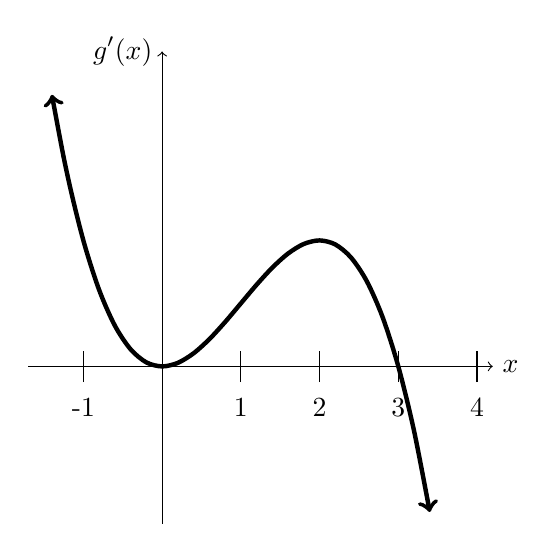
\begin{tikzpicture}[yscale=0.4,xscale=1]
  \draw[->] (-1.7, 0) -- (4.2, 0) node[right] {$x$};
  \draw[->] (0, -5) -- (0, 10) node[left] {$\displaystyle{g'(x)}$};
  \draw[<->, domain=-1.4:3.4, smooth, variable=\x, ultra thick] plot ({\x}, {\x*\x*(3-\x)});
  \foreach \i in {-1,1,2,3,4}{
  	\draw (\i,-.5)--(\i,0.5);
	\node at (\i,-1.3){\i};
	}
\end{tikzpicture}
\begin{subproblems}
	\item Determine the critical numbers of $g(x).$
	\vfill
	\quad
	\vfill
	\item  Determine the intervals on which $g(x)$ is increasing and intervals on which $g(x)$ is decreasing. 
	\vfill
	\quad\\
	\vfill
	\item  Identify the locations ($x$-values) of any extrema of $g(x).$ State the type of extrema (local/absolute maximum/minimum).
	\vfill
	\quad\\
	\vfill
	\item  Determine the intervals on which $g(x)$ is concave up and intervals on which $g(x)$ is concave down. 
	\vfill
	\quad\\
	\vfill
\end{subproblems}
\end{multicols}

\vspace{.5in}

\problem{6} Let $H(x)=\frac{2x+1}{x-9}$ 
\begin{subproblems}
\item Identify all vertical asymptotes or state that none exist. Justify your conclusion using limits.
\vfill
\item Identify all horizontal asymptotes or state that none exist. Justify your conclusion using limits.
\vfill
\end{subproblems}
\newpage
\problem{3} On the axes below, sketch a graph of $f(x)$ that satisfies all of the properties below:
\begin{multicols}{2}
(i) $f(0)=1$ \\
(ii) $f'(x) >0$ on $(-\infty,\infty)$\\
(iii) $f''(x) >0$ on $(-\infty,\infty)$

\begin{tikzpicture}[yscale=1,xscale=1]
  \draw[->] (-4.2, 0) -- (4.2, 0) node[right] {$x$};
  \draw[->] (0, -3) -- (0, 3) node[left] {$y$};
%   \foreach \i in {-3,-2,-1,1,2,3}{
%  	\draw (\i,-.1)--(\i,0.1);
%	\node at (\i,-1.3){\i};
%	}
\end{tikzpicture}
\end{multicols}


\problem{8} Evaluate the limits below. Use algebra to justify your answer. 
	\begin{subproblems}
	\item $\displaystyle \lim_{x \to -\infty} \frac{x^2+1}{x^2-2x^3}$
	\vfill
	\item $\displaystyle \lim_{x \to \infty} \frac{\sqrt{2x^4+x}}{1+x^2} $
	\vfill
	\end{subproblems}
\end{document}

